\FloatBarrier
\section{Design}
The Preshower Calorimeter (PCAL) is triangular in shape. The triangular form is isosceles in nature (not equilateral). This is done 
to better match the EC design and space limitations. A diagram of the side view of the PCAL with respect to the EC can be seen in 
Fig.~\ref{fig:geomfig1}. 

\begin{figure}[h]
    \centering
    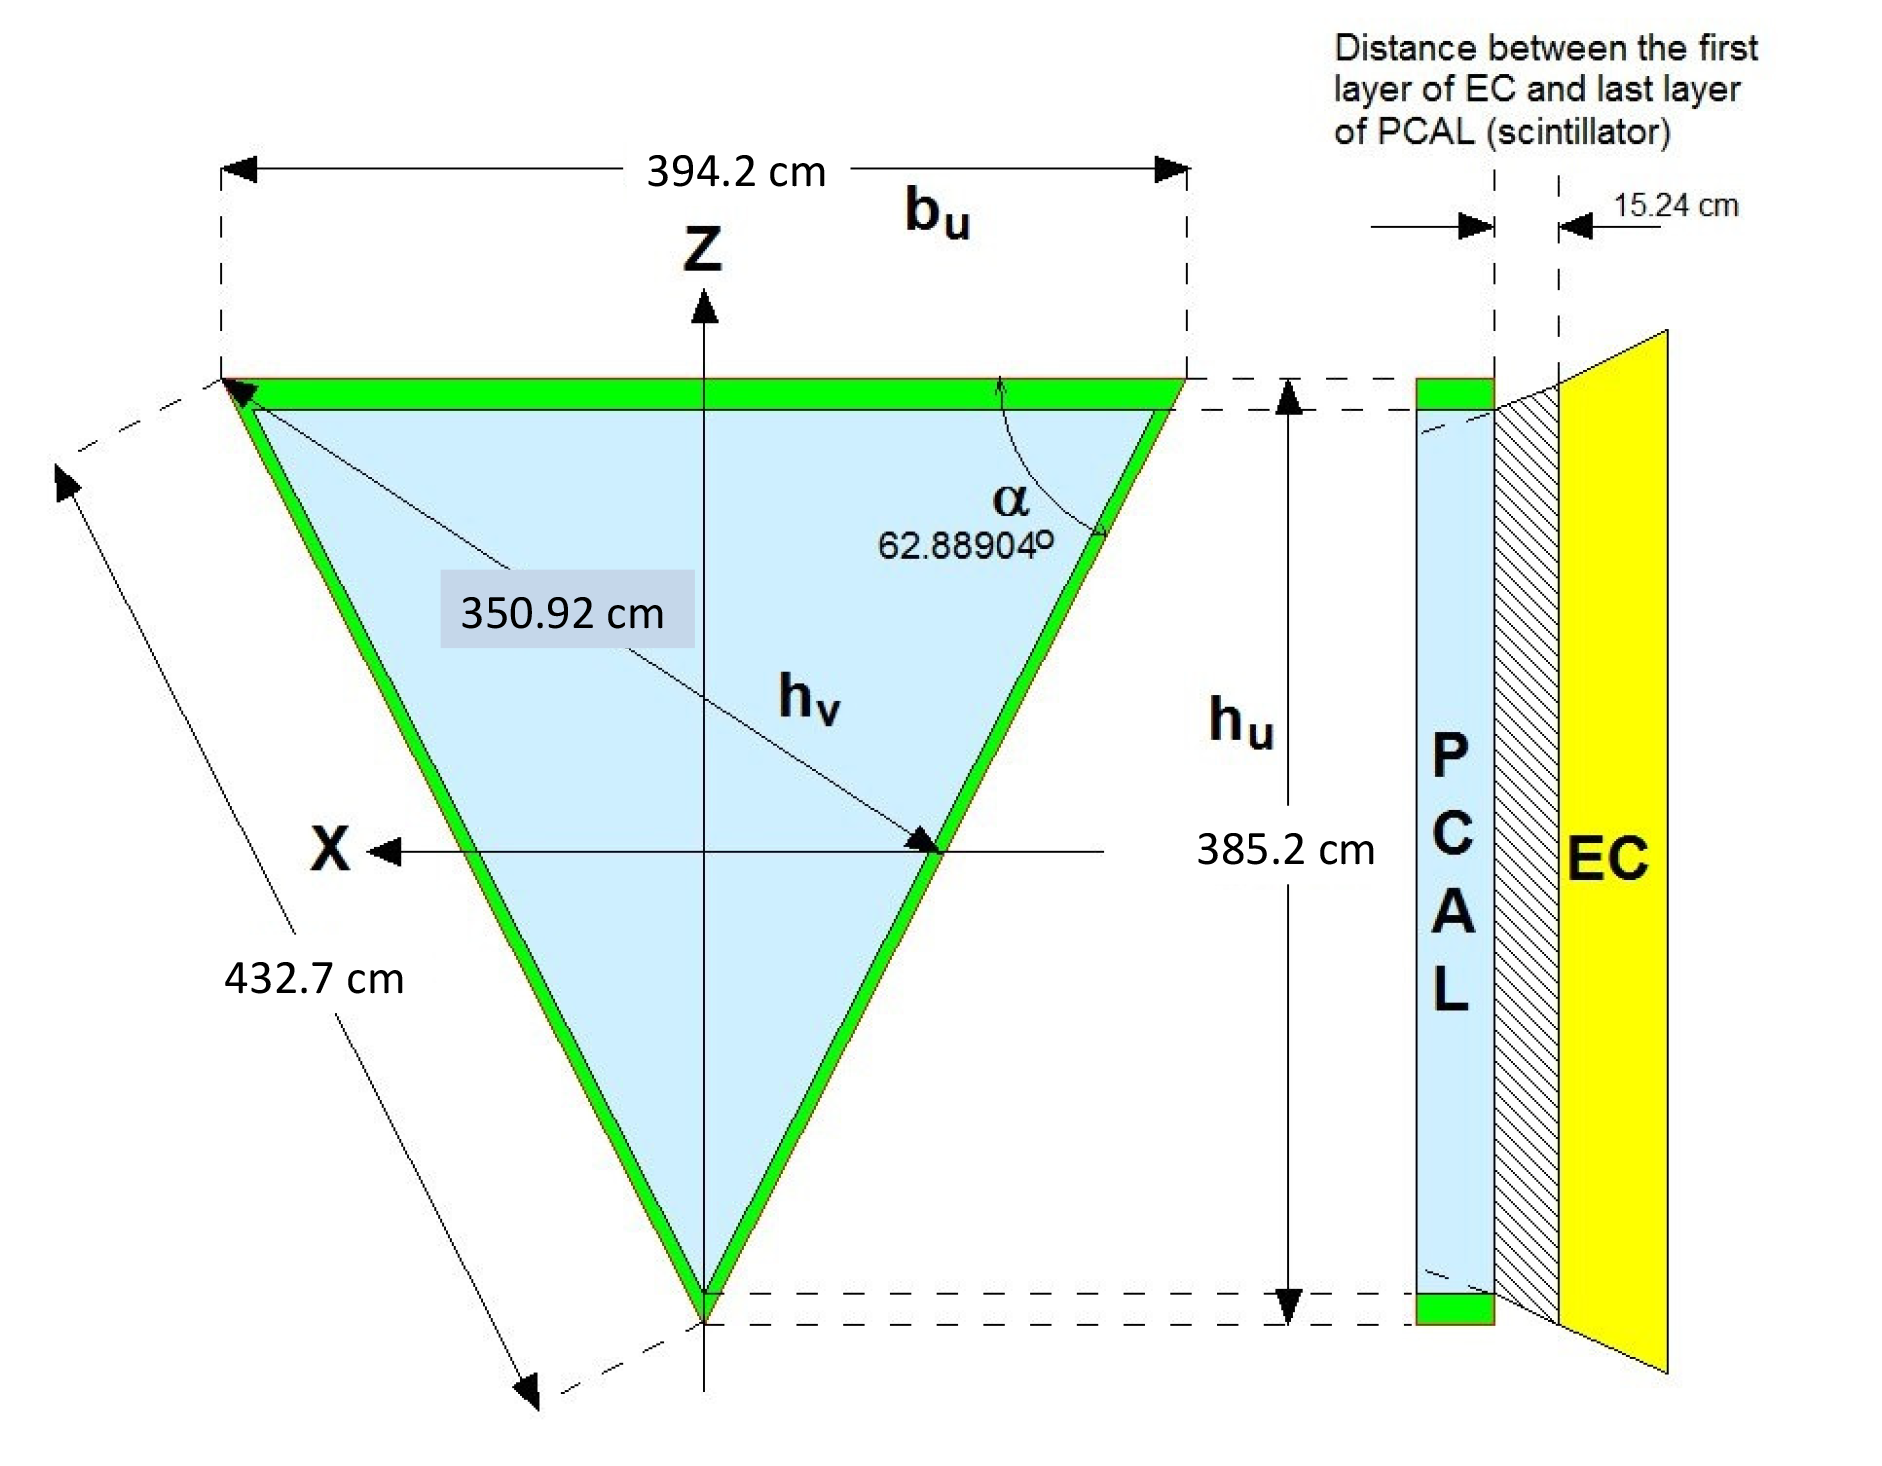
\includegraphics[width= 5in, keepaspectratio = true]{Pcal_geom_fig1}
    \caption{This diagram demonstrates the dimensions of the PCAL unit. This figure has been taken directly from the PCAL 
    geometry note\cite{bib:geomnote}.}
    \label{fig:geomfig1}
\end{figure}

The PCAL box encapsulates layers of scintillator strips and lead sheets. Between each lead sheet there are three different 
orientations of scintillating strips. These orientations are described as the U, V, and V layers. Each layer is parallel 
with one side of the PCAL box. The sequencing of the lead sheet, U layer, V layer, and W layer is repeated five times within
each sector of the PCAL unit. This results in fifteen layers of scintillator strips. Each repeating layer signal is coupled 
to the same PMT, and  is not able to separate five different signals. A UVW view of the PCAL can be seen in Fig.~\ref{fig:geomfig5}.

\begin{figure}[h]
    \centering
    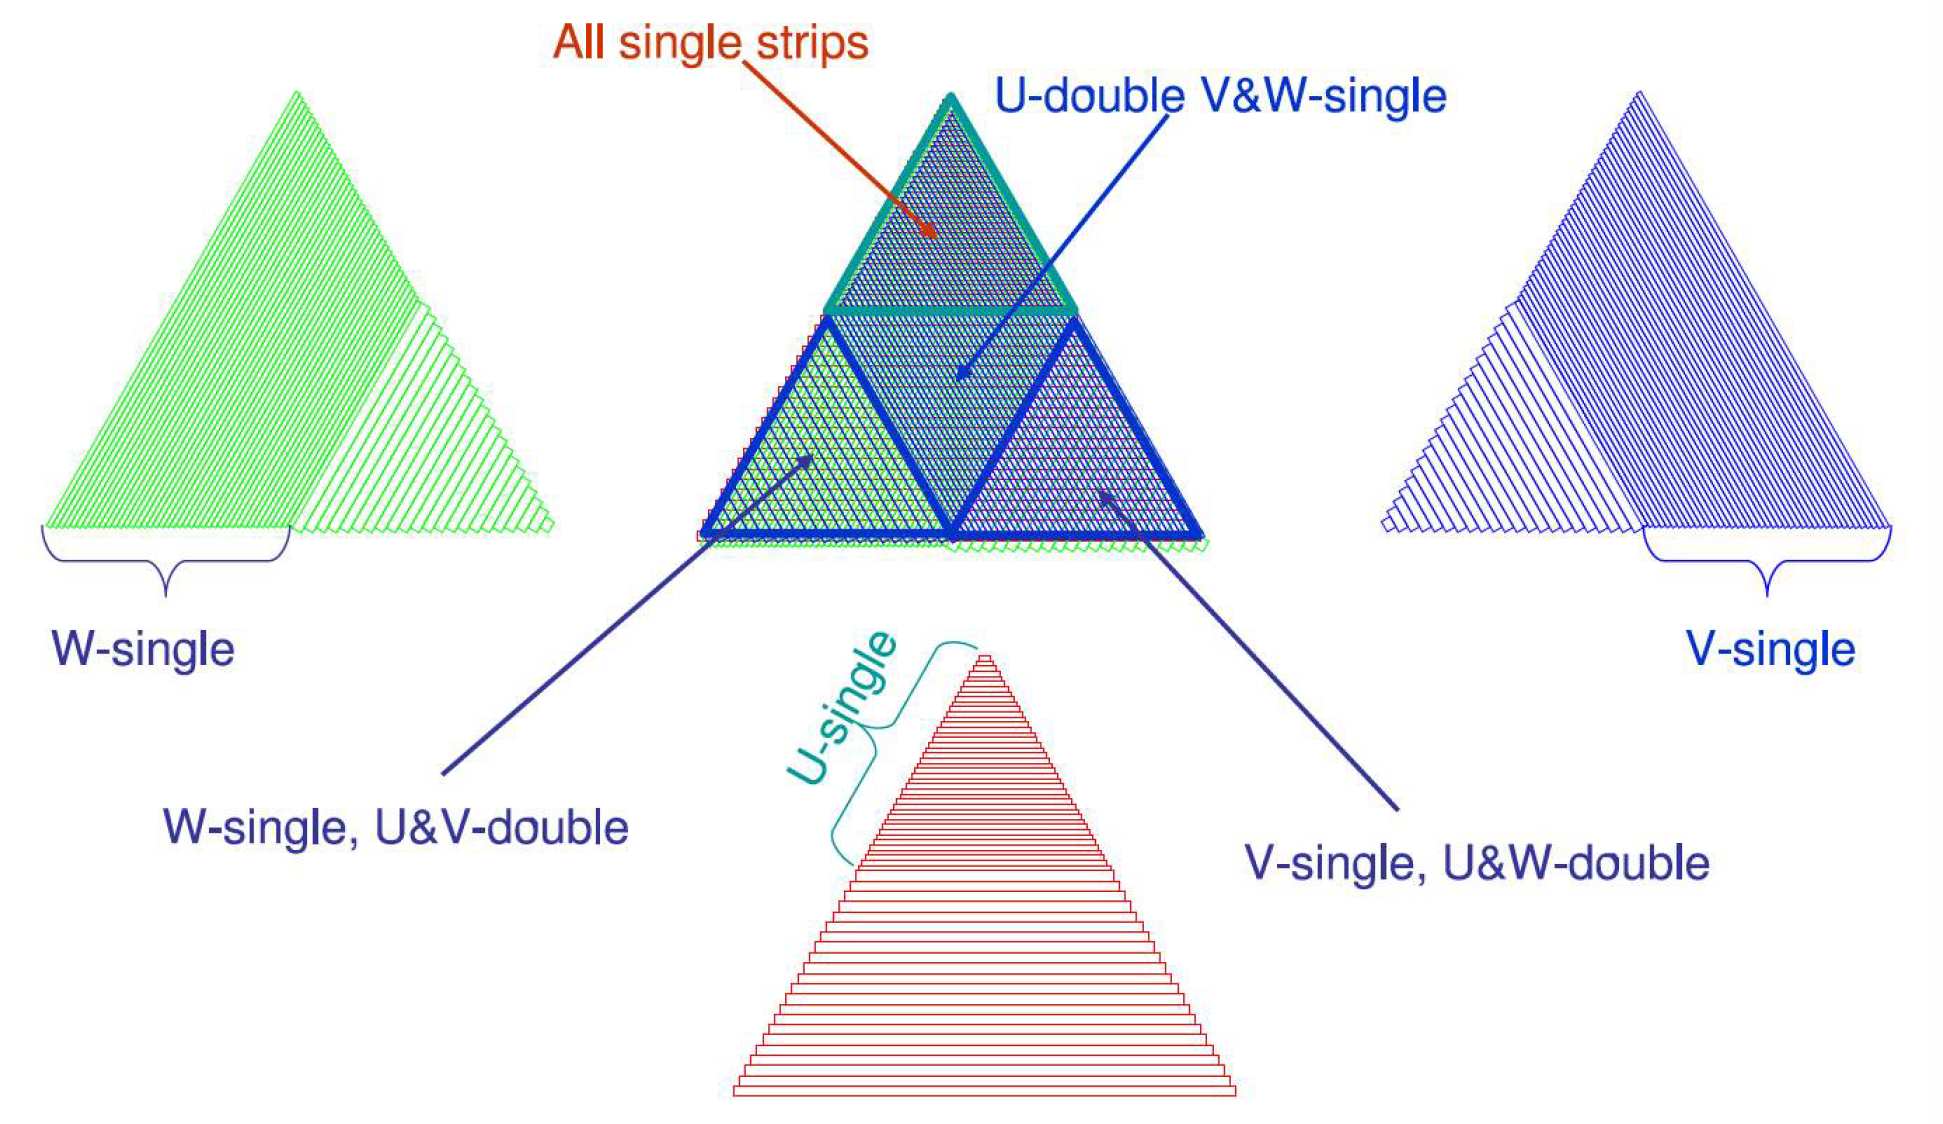
\includegraphics[width= 5in, keepaspectratio = true]{Pcal_geom_fig5}
    \caption{This is a schematic of how each orientation of scintillator is laid out. This figure is also taken directly from
     the PCAL geometry note\cite{bib:geomnote}.}
    \label{fig:geomfig5}
\end{figure}
\FloatBarrier

\FloatBarrier
There are 84 U strips, 77 V strips, and 77 W strips in each corresponding layer. The last 32 U strips are grouped into one PMT
per pair. The first 30 V and W strips are also grouped in pairs within their respective layer. As a consequence 
there is better spatial resolution at low strip numbers in the U layer and at high numbers in the V and W layers. This pattern 
of scintillators can be seen in Fig.~\ref{fig:geomfig5}.

Strips in each view can be numbered for ease. Lower numbered strips are the smaller strips while higher numbered strips are longer.
For example, V1 is the shortest and V62 is the longest strip in the V view. This strip convention is used throughout this
document and is taken from the PCAL geometry note\cite{bib:geomnote}. Using this convention, the layout of the PMT readout 
can easily be understood from Fig.~\ref{fig:PMTreadout} which shows PMT readout of a strip in each view. \textcolor{red}{The 
current analysis extracts calibration information based on 2-strip pixels only.}

\begin{figure}[h]
    \centering
    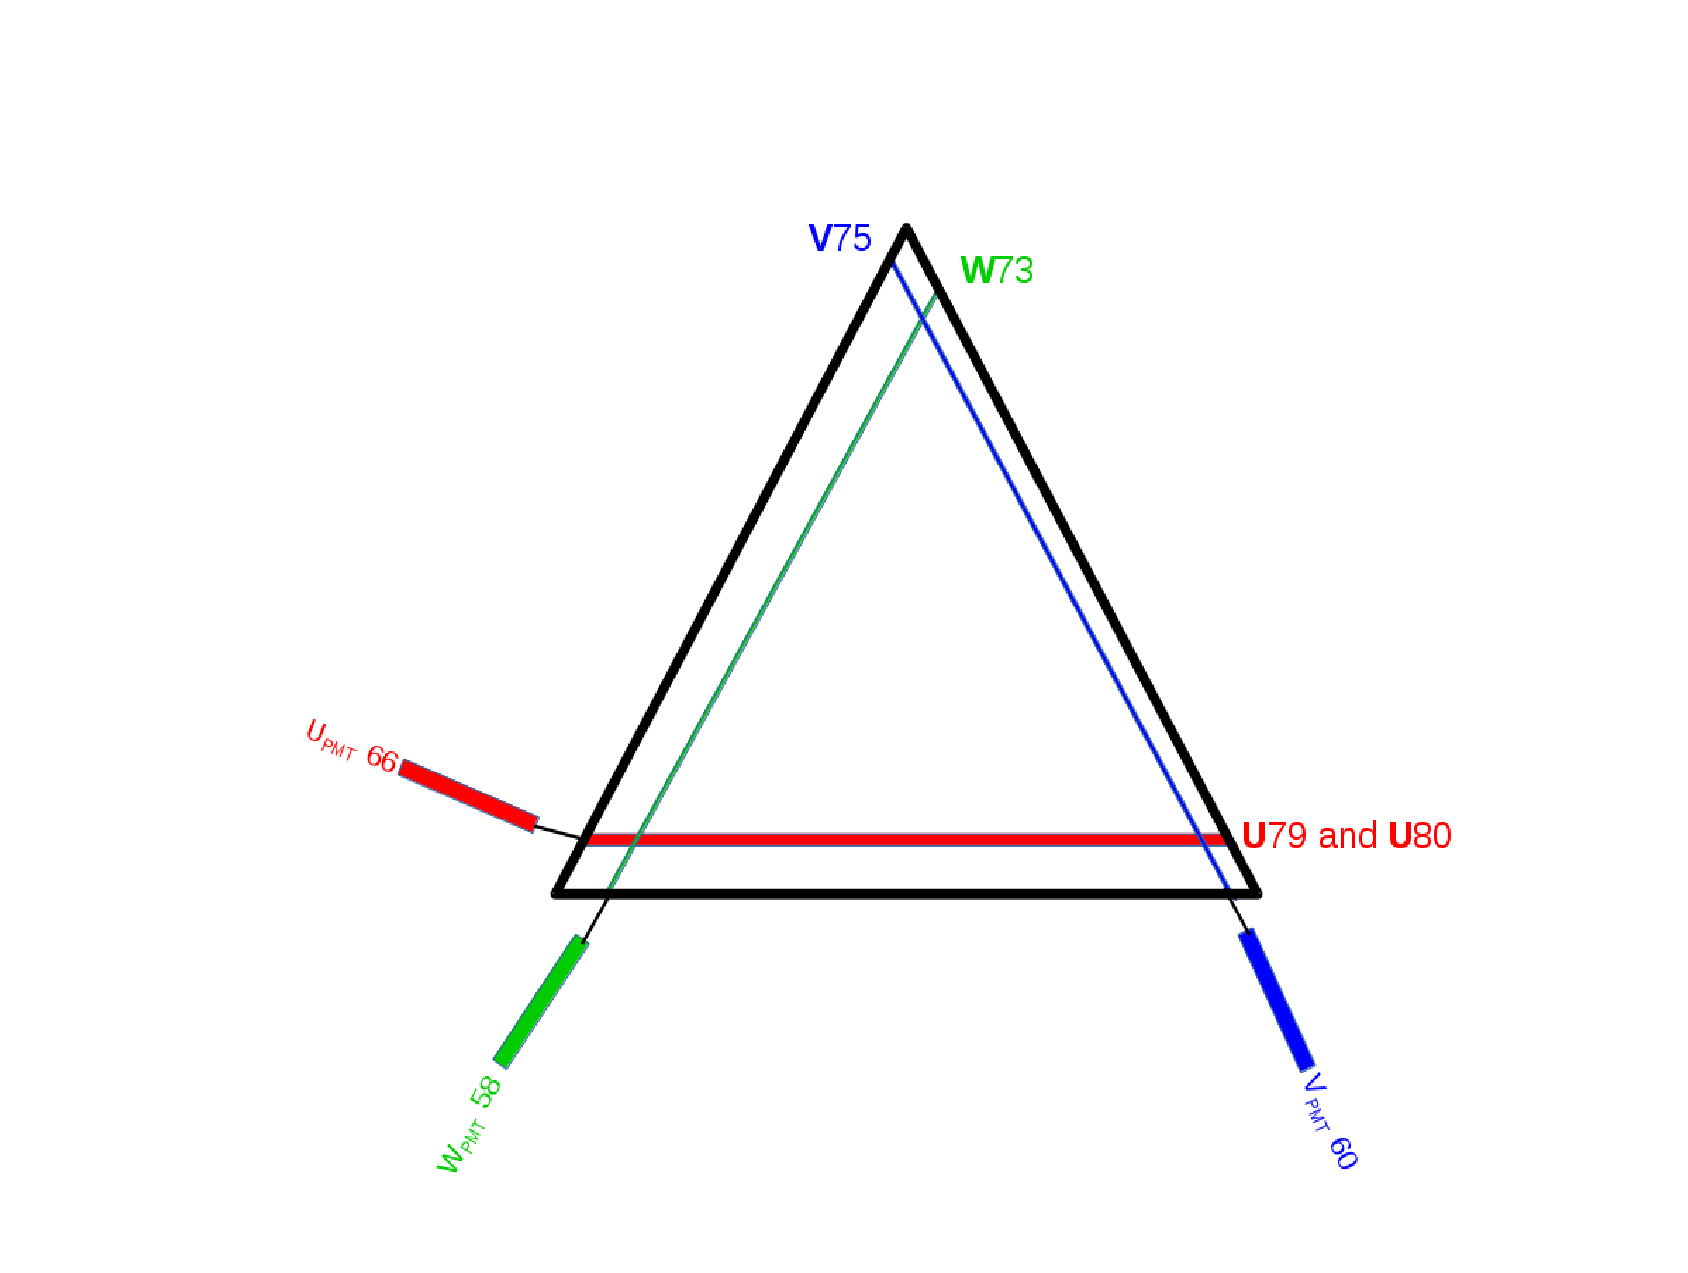
\includegraphics[width= 4.5in, keepaspectratio = true]{PMTreadout}
    \caption{This is a cartoon showing the layout of the PMT readout for different views.}
    \label{fig:PMTreadout}
\end{figure}
\FloatBarrier

\FloatBarrier
\subsection{Overlapping Shapes}
In order to calibrate the PCAL unit of the CLAS12 detector, one can think of dividing each PCAL module into bins based on the 
overlapping shapes. The overlap shapes/pixels are of two types: a 3-strip pixel, shape formed when all 
all the views are superimposed together, and a 2-strip pixel formed from the overlap of two strips where the strips are
part of different views. Maps of different overlap conditions are shown in Fig.~\ref{fig:PCAL_overlap}.


\begin{figure}[h]
  \centering
  \begin{subfigure}[b]{0.45\textwidth}
  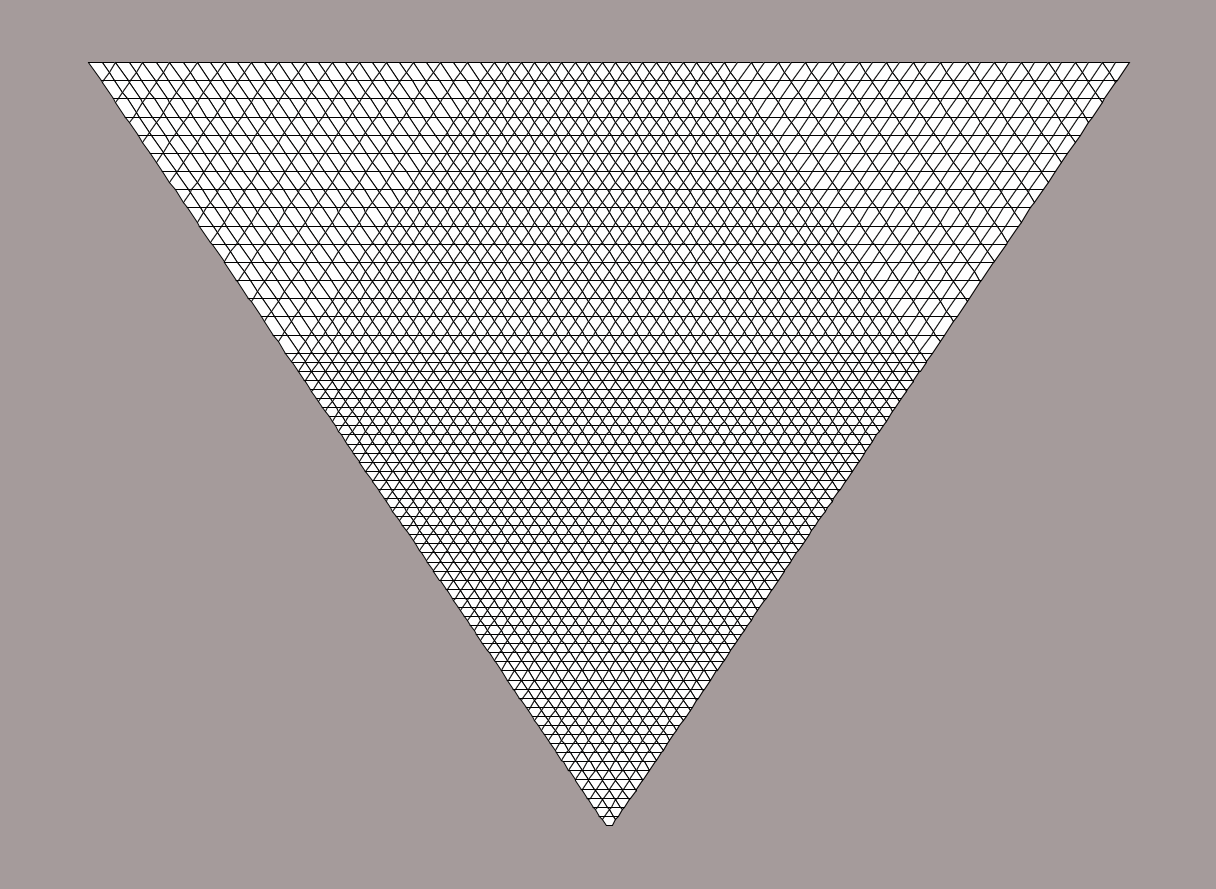
\includegraphics[width= 3in, keepaspectratio = true]{PCAL_pixel_screenshot}
  \caption{Pixel map.}
  %\label{fig:PCAL_pixel_screenshot}
  \end{subfigure}
  ~
  \begin{subfigure}[b]{0.45\textwidth}
  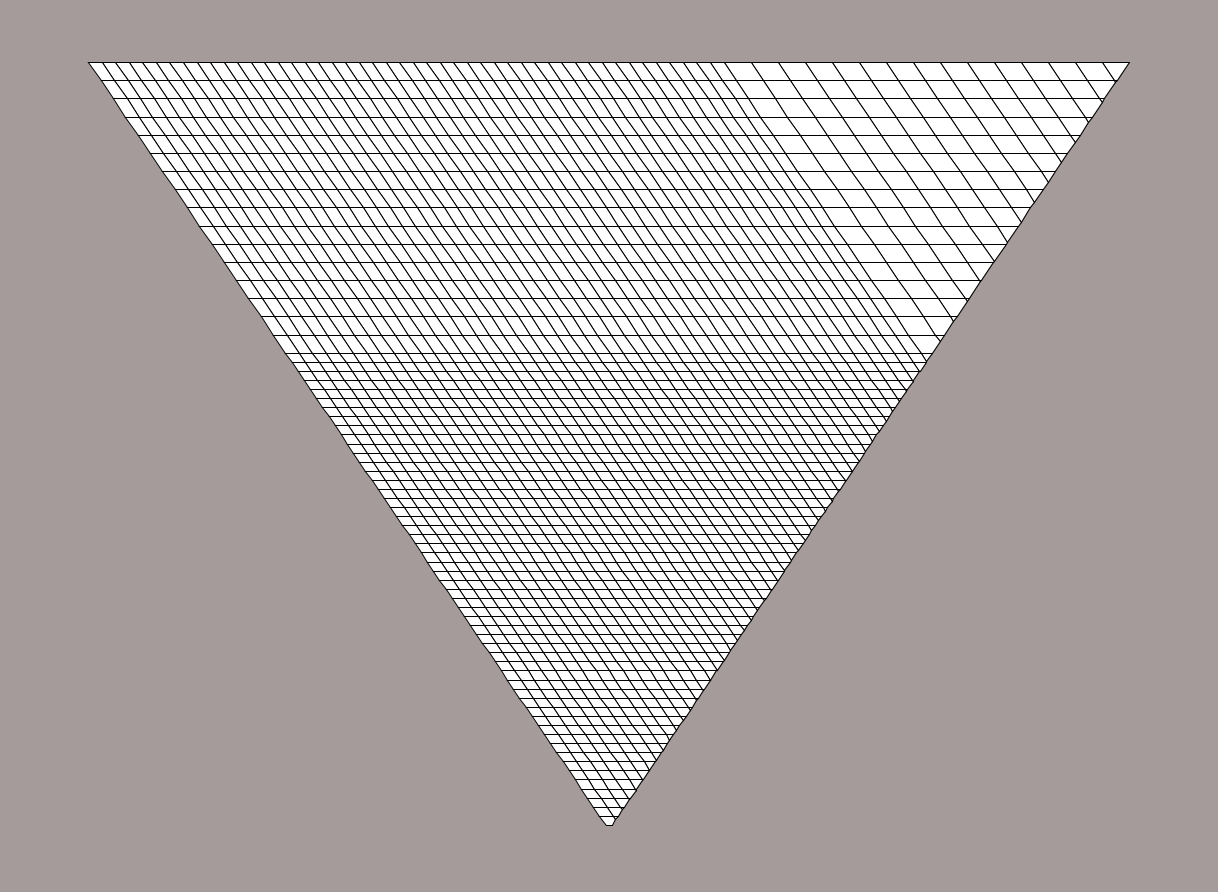
\includegraphics[width= 3in, keepaspectratio = true]{PCAL_UW_screenshot}
  %\caption{$M_{\pi^{+}\pi^{-}}$}
  %\label{fig:geomfig3b}
  \caption{UW overlap map.}
  %\label{fig:PCAL_UW_screenshot}
  \end{subfigure}

  \begin{subfigure}[b]{0.45\textwidth}
  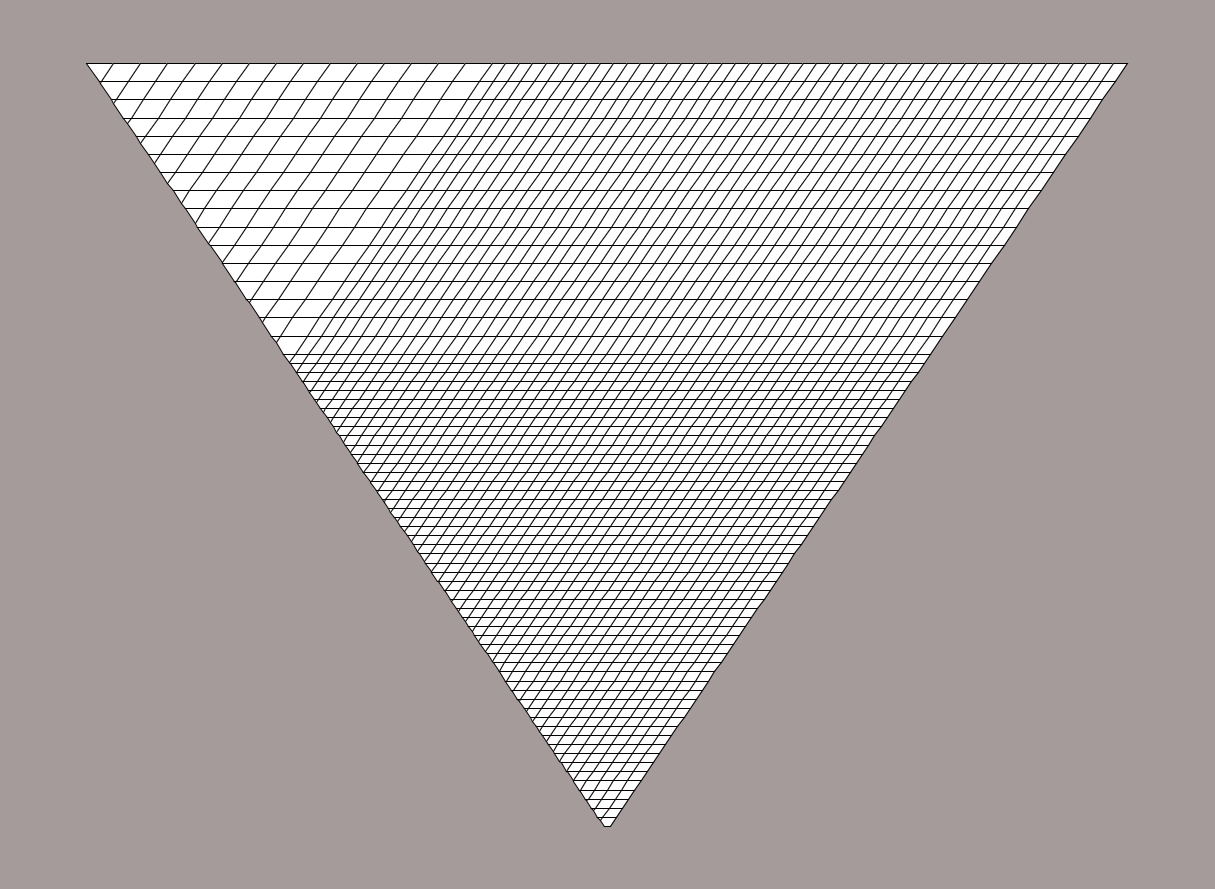
\includegraphics[width= 3in, keepaspectratio = true]{PCAL_UV_screenshot}
  %\caption{$M_{\pi^{+}\pi^{-}}$}
  %\label{fig:geomfig3b}
  \caption{UV overlap map.}
  %\label{fig:PCAL_UV_screenshot}
 \end{subfigure}
  ~
  \begin{subfigure}[b]{0.45\textwidth}
  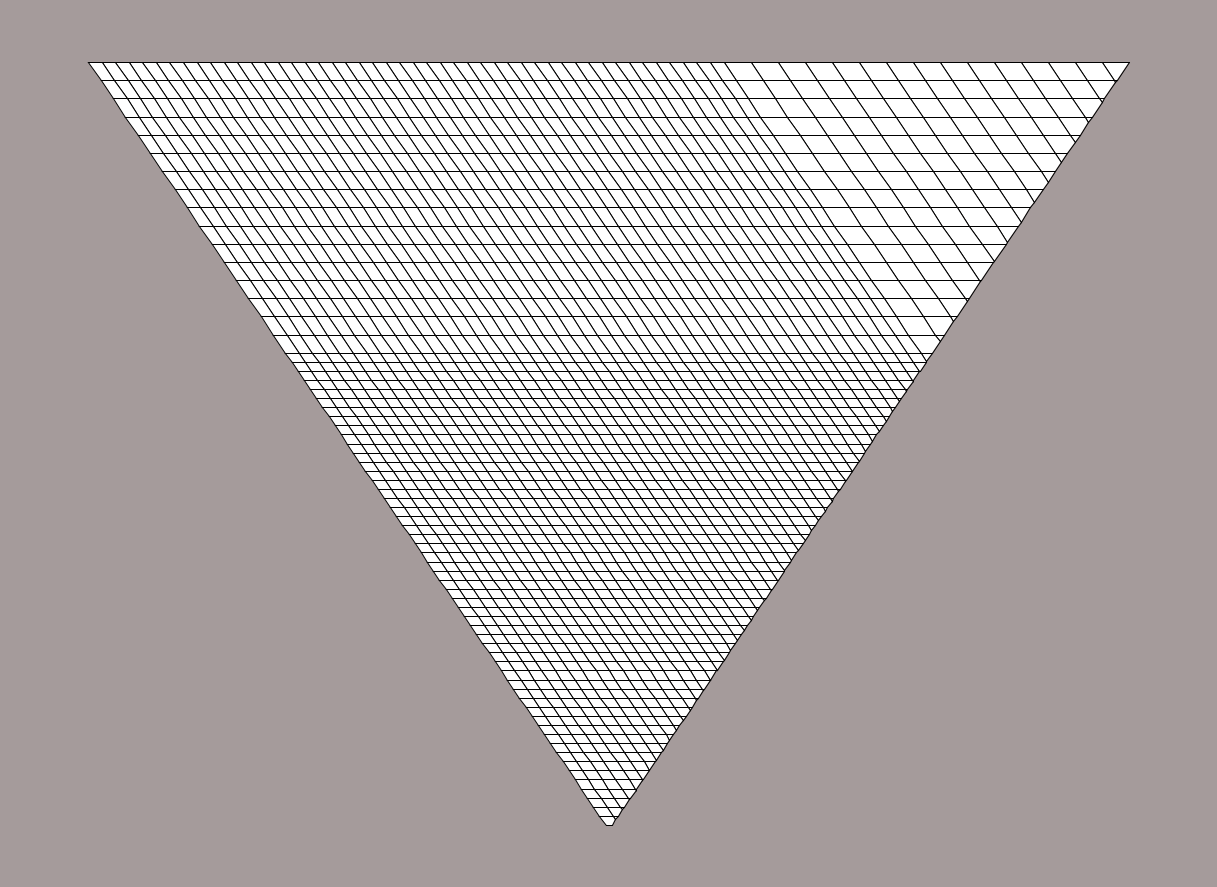
\includegraphics[width= 3in, keepaspectratio = true]{PCAL_WU_screenshot}
  \caption{WU overlap map.}
  %\label{fig:PCAL_WU_screenshot}
  \end{subfigure}
  ~
  \caption{Shown are the different ways overlaps can be considered in a single PCAL module.}
  \label{fig:PCAL_overlap}
\end{figure}
\FloatBarrier

\section{Data and Simulation}
The data used for the calibration was collected for the cosmic ray events before the PCAL unit was installed as a part of the CLAS12
detector subsystem. The collection required a trigger on the W-view meaning that information of cosmic ray tracks that created a PMT pulse of certain 
height were only stored. As the W-view is the last of the views, this trigger would also ensure to a reasonable level that the tracks
were perpendicular to the unit.

The calibration constants are extracted from simulated events as well to check the consistency of calibration code (based on \texttt{C++})
and the method used for the data. A \texttt{JAVA} framework is used for simulation and eventually the data. Details about the generation of 
simulated events and attenuation coefficients' extraction can be found in Section~\ref{Sec:simulation}.
\clearpage
